\documentclass[a4paper, fontsize=14pt]{article}
\usepackage[T2A]{fontenc}
\usepackage{mathtools}
\usepackage[utf8]{inputenc}
\usepackage[english, russian]{babel}
\usepackage{fancyhdr}
\usepackage{graphicx}
\usepackage{gensymb}
\usepackage{floatrow}
\usepackage{titlesec}
\usepackage{lastpage}
\usepackage{float}
\usepackage{gensymb}
\usepackage{booktabs}
\usepackage{amsmath}
\usepackage{amssymb}

\pagestyle{fancy}
	\fancyhf{}
	\lhead{\hspace{1bp} Работа \textnumero 3.2.5}
	\rhead{Терехов Максим 876\hspace{1bp}}
	\lfoot{Вынуждённые колебания в электрическом контуре}
	\cfoot{\textbf{}}
	\rfoot{\thepage\ \textnormal{из}\ \pageref{LastPage}}
	\renewcommand{\headrulewidth}{1pt}
	\renewcommand{\footrulewidth}{1pt}


%\addtolength{\hoffset}{-1.75cm}
%\addtolength{\textwidth}{3.5cm} 

%\addtolength{\voffset}{-1.5cm}
%\addtolength{\textheight}{3cm} 

\titleformat{\section}
    [block]{\normalfont\bfseries\large}{\rlap{\thesection}}{0em}
    {\vspace{-0.02\textwidth}\begin{minipage}[t]{.95\textwidth}}
[\end{minipage}]

\thispagestyle{fancy}

\begin{document}
\selectlanguage{russian}


\huge
\centering
\textbf{Вынуждённые колебания в электрическом контуре}

\raggedright
\parindent=1cm
\large
	\section*{Цель работы}
	Исследование вынужденных колебаний и процессов их установления.
	\section*{Оборудование}
	Генератор звуковой частоты (ЗГ), осциллограф (ЭО), вольтметр, частотометр, ёмкость, индуктивность, магазин сопротивлений, универсальный мост.
	\section*{Экспериментальная установка}
	\begin{figure}[H]
		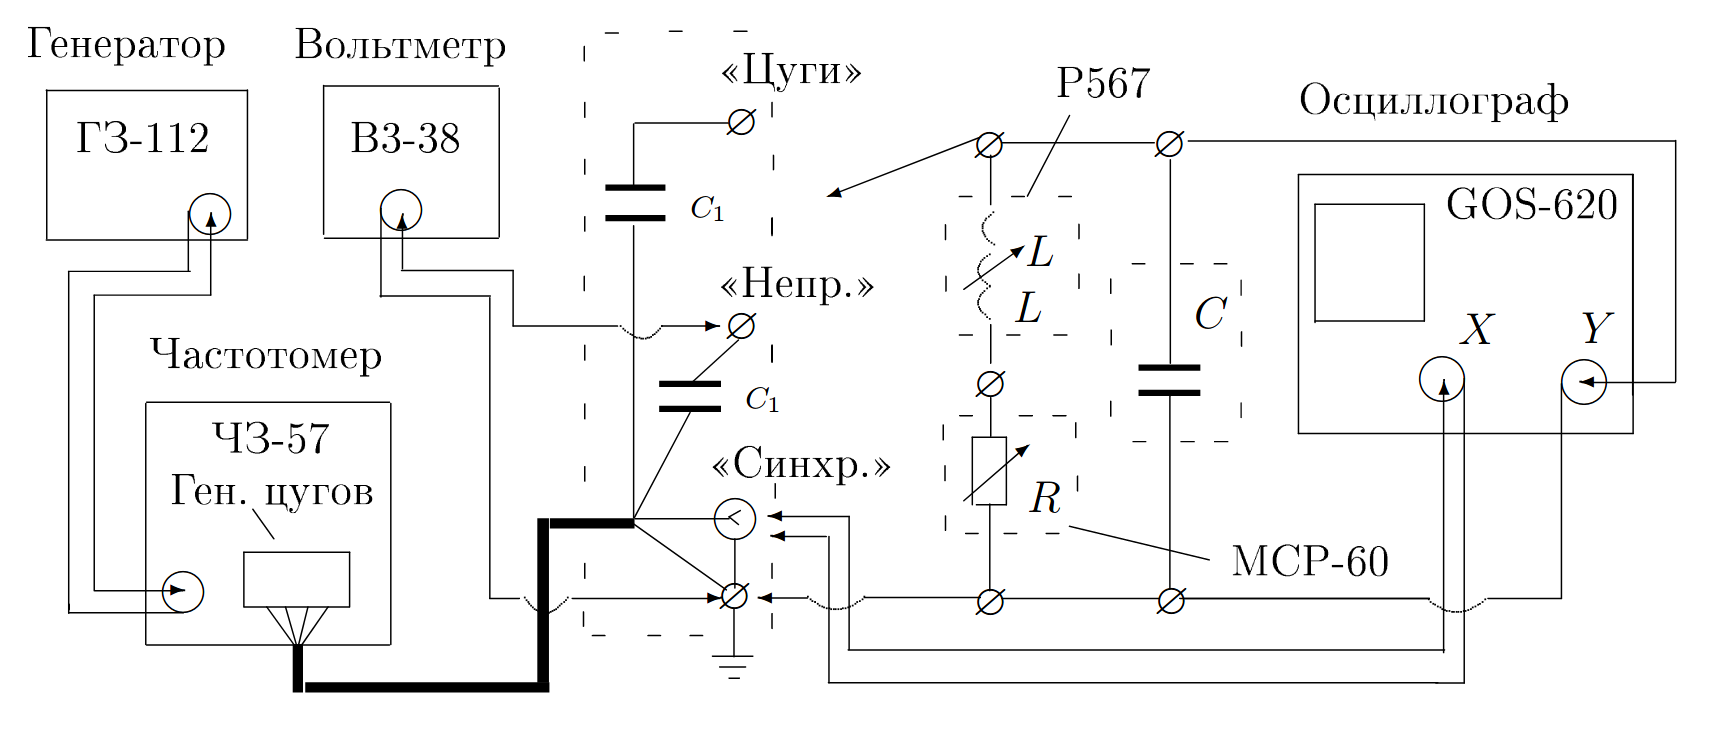
\includegraphics[width = 1.0\linewidth]{ust.png}
	\caption{Схема установки для исследования вынуждённых колебаний}
	\end{figure}
	\section*{Теоретическая часть}
	Для экспериментального исследования резонансной кривой тока в последовательном колебательном контуре можно снять зависимость амплитуды напряжения на резситоре $R$ от частоты генератора (при постоянной амплитуде выходного напряжения генератора). Но импеданс этого контура включает в себя выходной импеданс генератора. Мы должны быть уверены, что выходной импеданс генератора много меньше импеданса контура и не влияет на процессы, происходящие в этом контуре.
	
	Для устранения этого влияния можно использовать схему, представленную на рисунке (1): синусоидальный синал с генератора подаётся на параллельный колебательный контур через небольшую разделительную ёмкость $C_1$. Напряжение с ёмкости кнтура $C$ поступает на вертикальный вход ЭО.
	
	Зависимость амплитуды этого напряжения от частоты генератора будет практически совпадать с резонансной кривой для последовательного контура, если импедансы возбуждающей и измеряющей цепей (сопротивления переменному току) намного превосходят импеданс самого контура вблизи резонанса $Z_\text{рез} \approx L / (RC) = Q / (\Omega C)$. Разделительная ёмкость $C_1$ выбирается настолько малой, что в рабочем диапазоне частот её импеданс $Z_{C_1} = 1/(\Omega C_1)$ много меньше импеданса контура, поэтому в цепи генератора течёт ток практически с постоянной амплитудой, а колебательный контур выполняет роль нагрузочного сопротивления, которое, в свою очередь, зависит от частоты. Поскольку в резонансе сопротивление $Z_\text{рез}$ параллельного контура максимально, то и напряжение на ёмкости $C$ (неизменный ток, умноженный на максимальное сопротивление) тоже максимально. Входное сопротивление осциллографа (измеряющей цепи) достаточно велико: $R_\text{ЭО} \approx 1 \text{МОм}$.
	
	Таким образом, при выполнении условий
	\[
		Z_{C_1} = \frac{1}{\Omega C_1} \gg |Z| = \frac{Q}{\Omega C}, \quad R_\text{ЭО} \gg \frac{Q}{\Omega C}
	\]
	и при условии, что действительная часть импеданса катушки много меньше её мнимой части, резонансная кривая в нашем контуре бует выглядеть так же, как в последовательном: максимум амплитуды при резонансе. Ширина резонансной кривой определяет важную характеристику контура --- добротность.
	
	Добротность контура может быть определена и другими способами, например, по скорости нарастания амплитуды вынужденных колебаний при резонансе или по скорости затухания свободных колебаний. Нарастание и затухание колебаний можно наблюдать на экране осциллографа, если на контур подаются цуги --- отрезки синусоиды, разделённые интервалами, в течение которых сигнал отсутствует. Чем выше добротность, тем медленне нарастают и медленнее затухают колебания в контуре. Количественные оценки можно сделать, сли определить логарифмический декремент затухания по скорости нарастания или затухания колебаний. В условиях резонанса огибающая затухающих колебаний это перевёрнутая огибающая нарастающего участка, поэтому при расчёте логарифмического декремента по затуханию нет необходимости использовать амплитуду установившихся колебаний $U_0$, которая в контуре с высокой добротностью иногда не успевает установиться за время продолжительности цуга.
	\section*{Обработка результатов измерений}
	Теоретическая и найденная экспериментально резонансная частота:
	\[
	\nu_0 = 1575\ \text{Гц}; \quad \nu_{0_\text{теор}} = \frac{1}{2 \pi \sqrt{LC}} = 1592.4\ \text{Гц}
	\]
\begin{figure}[H]
	\begin{floatrow}
	\ttabbox{\caption{Измерения при $R = 100$ Ом}}{	
	\begin{tabular}{|c|c|} \hline
$\nu,\ \text{кГц}$ & $U, B$ \\\hline
1.522 &   7.2 \\\hline
1.530 &   8.4 \\\hline
1.537 &   9.4 \\\hline
1.540 &  10.0 \\\hline
1.548 &  12.0 \\\hline
1.555 &  14.0 \\\hline
1.561 &  16.0 \\\hline
1.567 &  18.0 \\\hline
1.575 &  18.6 \\\hline
1.581 &  18.0 \\\hline
1.587 &  16.0 \\\hline
1.593 &  14.0 \\\hline
1.600 &  12.0 \\\hline
1.608 &  10.0 \\\hline
1.613 &   9.6 \\\hline
1.618 &   8.8 \\\hline
1.627 &   7.6 \\\hline
1.634 &   6.8 \\\hline
	\end{tabular}}	
\ttabbox{\caption{Измерения при $R = 0$ Ом}}{
	\begin{tabular}{|c|c|} \hline
$\nu,\ \text{кГц}$ & $U, B$ \\\hline
1.360 &  1.40 \\\hline
1.408 &  1.80 \\\hline
1.443 &  2.20 \\\hline
1.468 &  2.60 \\\hline
1.493 &  3.00 \\\hline
1.516 &  3.40 \\\hline
1.538 &  3.80 \\\hline
1.551 &  4.00 \\\hline
1.575 &  4.15 \\\hline
1.616 &  3.90 \\\hline
1.653 &  3.40 \\\hline
1.682 &  3.00 \\\hline
1.700 &  2.80 \\\hline
1.717 &  2.60 \\\hline
1.742 &  2.40 \\\hline
1.766 &  2.20 \\\hline
1.794 &  2.00 \\\hline
1.841 &  1.80 \\\hline
1.887 &  1.60 \\\hline
1.955 &  1.40 \\\hline
2.055 &  1.20 \\\hline
\end{tabular}}
\end{floatrow}
\end{figure}

\begin{figure}[H]
	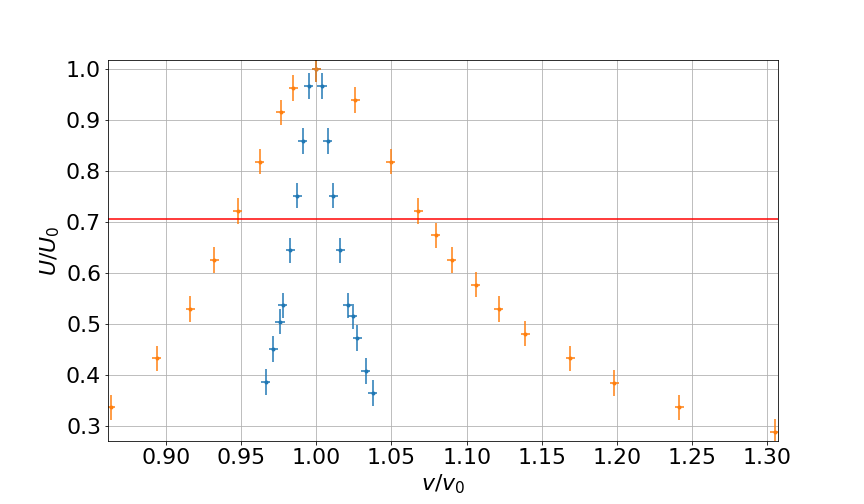
\includegraphics[width = 1.0\linewidth]{10.png}
\caption{График зависимости $U / U_0$ от $\nu / \nu_0$}
\end{figure}
Найдём добротность из графика по формуле:
\[
	Q = \frac{\omega_0}{2 \Delta \Omega}
\]
\[
	Q_0 = 25 \pm 1 \quad Q_{100} = 7.6 \pm 0.5 
\]
Рассчитаем добротность контура по скорости нарастания и затухания колебаний:
	\begin{figure}[H]
		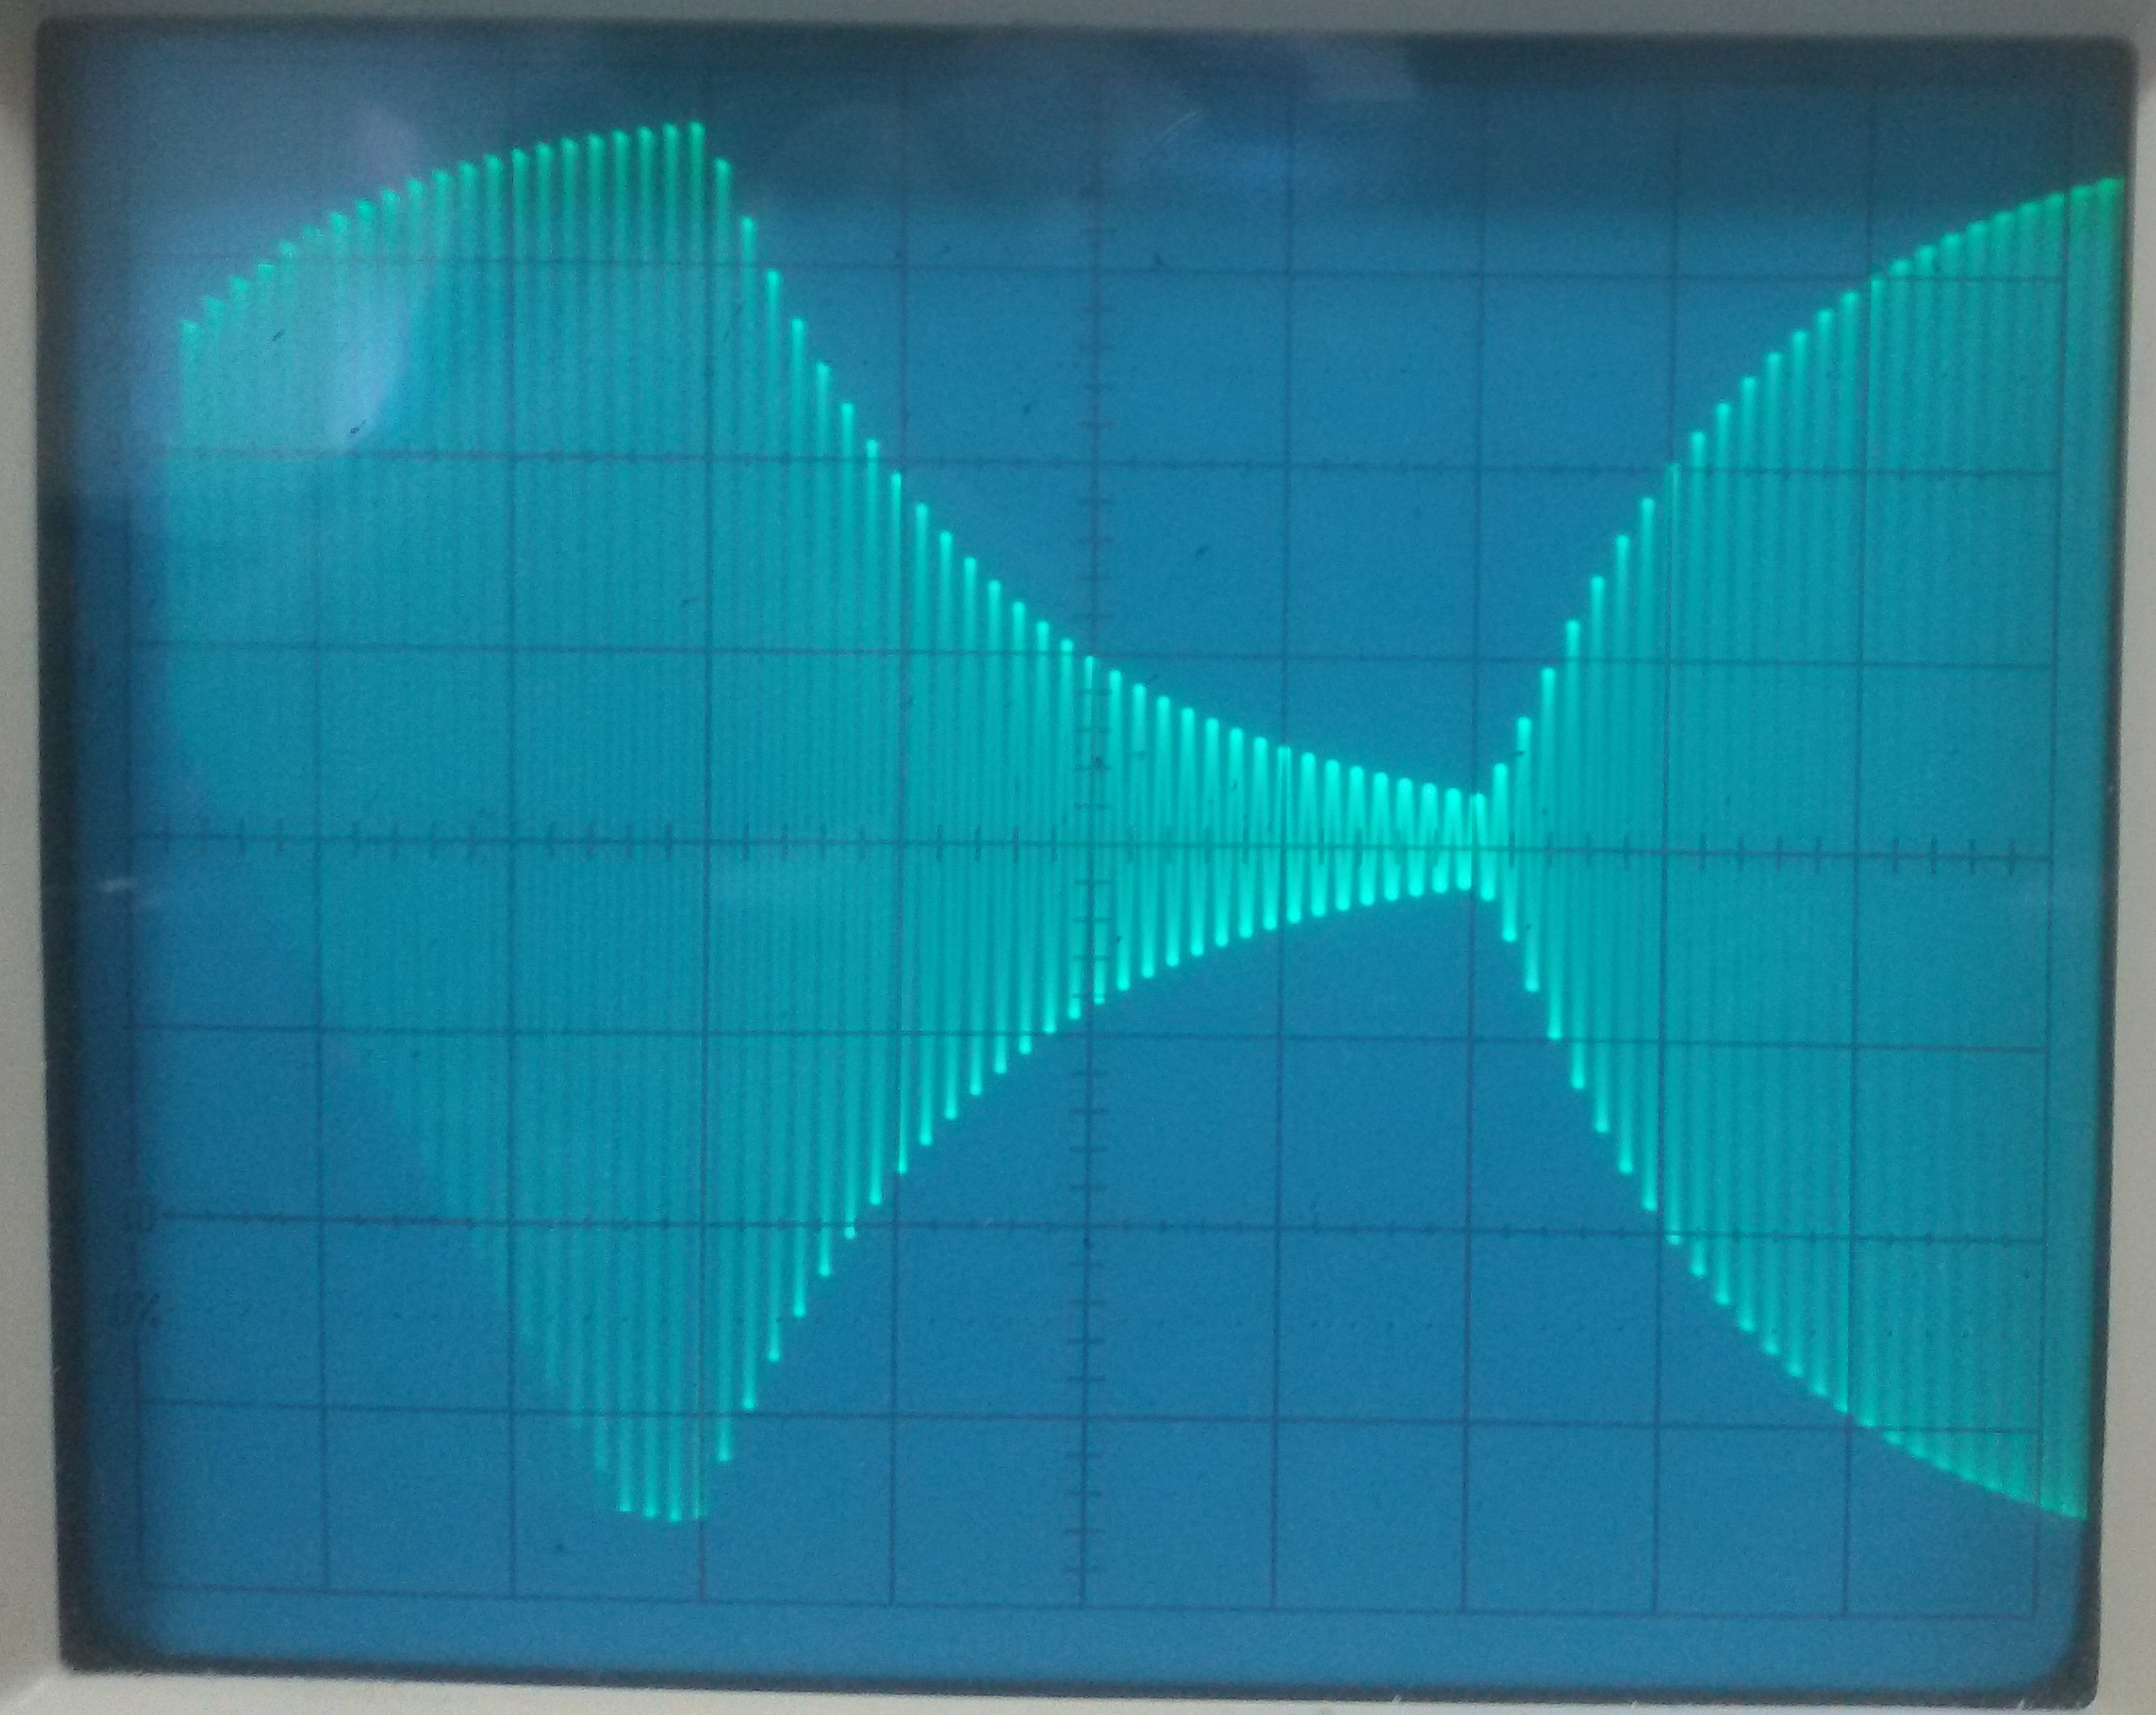
\includegraphics[width = 0.88\linewidth]{zug.jpg}
	\caption{Нарастание и затухание колебаний}
	\end{figure}
	\begin{table}[H]
	\centering
	\begin{tabular}{|c|c|c|c|c|c|c|c|c|}  \hline
	{} & \multicolumn{4}{|c|}{Нарастание} & \multicolumn{4}{|c|}{Затухание} \\\hline
	$U_k,\ \text{дел}$ & 12 & 12 & 14 & 20 & 30 & 29 & 29 & 28 \\\hline
	$U_{k+n}, \text{дел}$ & 14 & 20 & 26 & 30 & 27 & 24 & 26 & 23 \\\hline
	$n$ & 1 & 4 & 7 & 8 & 3 & 4 & 3 & 4 \\\hline
	$Q$ & 36.1 & 30.9 & 27.9 & 25.6 & 25.2 & 23.3 & 26.4 & 25.9 \\\hline
	$\sigma Q$ & 2.8 & 2.4 & 2.0 & 2.1 & 1.7 & 1.6 & 1.7 & 1.7 \\\hline
	\end{tabular}
	\caption{Данные нарастаний и затуханий цуги при $R = 0\ \text{Ом}$}
	\end{table}

	\begin{table}[H]
	\centering
	\begin{tabular}{|c|c|c|c|c|c|c|c|c|}  \hline
	{} & \multicolumn{4}{|c|}{Нарастание} & \multicolumn{4}{|c|}{Затухание} \\\hline
	$U_k,\ \text{дел}$ & 10 & 19 & 28 & 33 & 32 & 27 & 33 & 37 \\\hline
	$U_{k+n}, \text{дел}$ & 18 & 32 & 36 & 38 & 15 & 9 & 9 & 5 \\\hline
	$n$ & 2 & 2 & 2 & 2 & 2 & 2 & 3 & 5 \\\hline
	$Q$ & 7.6 & 7.6 & 7.4 & 7.7 & 6.3 & 8.7 & 7.3 & 7.8 \\\hline
	$\sigma Q$ & 1.1 & 1.0 & 0.9 & 0.9 & 0.7 & 1.1 & 1.0 & 1.1 \\\hline
	\end{tabular}
	\caption{Данные нарастаний и затуханий цуги при $R = 100\ \text{Ом}$}
	\end{table}

	\begin{table}[H]
	\centering
	\begin{tabular}{|c|c|c|} \hline
	$R,\ \text{Ом}$ & $Q_\text{воз}$ & $Q_\text{зат}$ \\\hline
	$0$ & $30.1 \pm 2.2$ & $25.2 \pm 1.8$ \\\hline
	$100$ & $7.5 \pm 0.9$ & $7.5 \pm 0.9$ \\\hline 
	\end{tabular}	
	\end{table}
	\section*{Вывод}
	\[
		Q_\text{теор} = R \sqrt{\frac{C}{L}}
	\]
	\begin{table}[H]
	\centering
	\begin{tabular}{|c|c|c|c|c|c|} \hline
	$R,\ \text{Ом}$ & $R_\text{акт},\ \text{Ом}$ & $Q_\text{граф}$ & $Q_\text{воз}$ & $Q_\text{зат}$ & $Q_\text{теор}$ \\\hline
	$0$ & $25.075$ & $25 \pm 1$ & $30.1 \pm 2.2$ & $25.2 \pm 1.8$ & $25.7 \pm 1$ \\\hline
	$100$ & $25.075$ & $7.6 \pm 0.5$ & $7.5 \pm 0.9$ & $7.5 \pm 0.9$ & $7.7 \pm 0.5$ \\\hline 
	\end{tabular}	
	\end{table}
	Полученное экспериментально значение добротности с учетом погрешности совпадает с теоретическим. Метод определения доротности по графику даёт довольно точные результаты.
\end{document}